% Created 2020-10-26 一 20:58
% Intended LaTeX compiler: xelatex
\documentclass[11pt]{article}
\usepackage{graphicx}
\usepackage{grffile}
\usepackage{longtable}
\usepackage{wrapfig}
\usepackage{rotating}
\usepackage[normalem]{ulem}
\usepackage{amsmath}
\usepackage{textcomp}
\usepackage{amssymb}
\usepackage{capt-of}
\usepackage{hyperref}
\usepackage[scheme=plain]{ctex}
\usepackage{fontspec}
\setmainfont{更纱黑体 UI SC}
\hypersetup{colorlinks=true,linkcolor=blue}
\usepackage{longtable}
\author{曹嘉祺 PB18030874}
\date{\today}
\title{乙酸乙酯皂化反应动力学研究}
\hypersetup{
 pdfauthor={曹嘉祺 PB18030874},
 pdftitle={乙酸乙酯皂化反应动力学研究},
 pdfkeywords={乙酸乙酯皂化反应 速率常数 电导率 活化能 反应级数},
 pdfsubject={},
 pdfcreator={Emacs 27.1 (Org mode 9.4)}, 
 pdflang={English}}
\begin{document}

\maketitle
\begin{abstract}


实验中分别测定了30°C和35°C恒温下乙酸乙酯和氢氧化钠的混合溶液在不同时刻的
电导率值, 从而计算出在30°C时的反应速率常数k\textsubscript{1}和35°C时的反应速率常数k\textsubscript{2}。 并且
由阿仑尼乌斯经验公式求得反应的活化能E\textsubscript{a}。 从而了解具有简单级数的化学反应的动
力学特征, 并熟悉了电导率仪的使用方法。

\begin{itemize}
\item 关键词: 乙酸乙酯皂化反应, 速率常数, 电导率, 活化能, 反应级数
\end{itemize}
\end{abstract}
\section{前言}
\label{sec:org758edcf}
化学动力学的基本任务之一是了解反应的速率,了解各种因素(如分子结构、温度、
压力、浓度、介质、催化剂等)对反应速率的影响;另一个基本任务是研究反应历程。所谓
反应历程,就是反应物究竟按什么途径、经过哪些步骤才转化为最终产物\textsubscript{[1]}。
反应速率常数是化学反应一个重要的动力学参数。根据实验原理,在其一恒定温度下,
只要氢氧化钠与乙酸乙酯的初始浓度相等,就必然有下式成立\textsubscript{[2]}:
\[
\frac{L_{0}-L_{t}}{L_{t}-L_{\infty}}=akt
\]
要测定化学反应速率,必须测出在不同反应时刻的反应物(或生成物)的浓度,绘制出物质浓度随
时间的变化的血线,然后从图上求出不同反应时刻的速率。

测定反应物(或生成物)在不同反应时刻的浓度一般可用化学方法和物理方法。化学方
法是在某一时刻出取一部分物质,并设法迅速使反应停止。然后进行化学分析,这样可直接
得到不同时刻某物质浓度的数值,但实验操作则往往较繁;物理方法是在反应过程中,对某
一种与物质浓度有关的物理量进行连续监测,获得一些原位反应的数据。

乙酸乙酯皂化反应中,固导电离子浓度随反应时间变化而变化,因此可用电导率仪测
量皂化反应进程中电导率随时间的变化,从而达到跟踪反应物浓度随时间变化的目的,经过
作图和数据处理 可得到反应的反应速率常数。

乙酸乙酯皂化反应是一个在化学和工业应用上均有着重大意义的有机反应,此实验通
过对其反应速率的研究,确定反应速率常数,并进一步测定出该反应的活化能。不同时刻各
物质的浓度可用化学分析法测出,例如分析反应中的 OH\textsuperscript{-} 浓度,也可用物理电导法测量溶
液的电导而求出。在本实验中我们采用电导法来测定。


\section{实验部分}
\label{sec:orge6ac875}
\subsection{主要化学试剂}
\label{sec:orge49c772}
\begin{center}
\begin{tabular}{lrll}
试剂 & 分子量 & 试剂规格 & 生产商\\
\hline
NaOH & 40.01 & AR & 国药集团化学试剂有限公司\\
乙酸乙酯 & 88.11 & AR & 国药集团化学试剂有限公司\\
邻苯二甲酸氢钾 & 204.23 &  & \\
酚酞 &  &  & \\
\end{tabular}
\end{center}

\subsection{主要仪器设备}
\label{sec:orgcea5e40}
\begin{center}
\begin{tabular}{lrl}
仪器 & 数目 & 生产商\\
\hline
DDS-型电导率仪 & 1 & SevenMulti\\
HK-2A 超级恒温水浴 & 1 & 南京大学应用物理研究所监制\\
JB-1B 型磁力搅拌器 & 1 & 上海雷磁新径仪器有限公司\\
电导池 & 1 & \\
100mL 恒温夹套反应器 & 1 & \\
0. 2mL,100ml 移液管 & 1 & \\
50mL 的烧杯 & 1 & \\
50mL 滴定管 & 1 & \\
250mL 锥形瓶 & 3 & \\
吸耳球 & 1 & \\
\end{tabular}
\end{center}

\subsection{实验原理}
\label{sec:org062f04c}
化学反应动力学研究的两个方面为:
\begin{enumerate}
\item 化学反应速率研究
\item 化学反应机理(或历程)研究
\end{enumerate}

乙酸乙酯皂化反应方程式为:
\[
CH_3COOC_2H_5+Na^+ + OH^- ══ CH_3COO^- + Na^+ +C_2H_5OH
\]
在反应过程中,各物质的浓度随时间而改变(注:Na\textsuperscript{+}
离子在反应前后浓度不变)。若
乙酸乙酯的初始浓度为 a,氢氧化钠的初始浓度为 b,当时间为 t 时,各生成物的浓度均为 x,
此时刻的反应速度为:
\[
\frac{dx}{dt}=k(a-x)(b-x)
\]
式中,k 为反应的速率常数,将上式积分可得:
\[
kt=\frac{1}{a-b}ln\frac{b(a-x)}{a{b-x}}
\]

若初始浓度 a=b,上式变为
\[
\frac{dx}{dt}=k(a-x)^2
\]
积分得
\[
kt=\frac{x}{a(a-x)}
\]
不同时刻各物质的浓度可用化学分析法测出,例如分析反应中的 OH\textsuperscript{-}
浓度,也可用物
理法测量溶液的电导而求得。在本实验中我们采用后一种方法,即用电导法来测定。

电导是导体导电能力的量度,金属的导电是依靠自由电子在电场中运动来实现的,而电
解质溶液的导电是正、负离子向阳极、阴极迁移的结果,电导 L 是电阻 R 的倒数。
\[
L=\frac{1}{R}=L_{g}\frac{A}{l}
\]
式中 A 为导体的截面积,l 为导体的长度,L\textsubscript{g} 称电导率。
它的物理意义是:当 l=1m,A=1m\textsuperscript{2}
时的电导。对一种金属,在一定温度下, L\textsubscript{g} 是一定的。
对电解质溶液的 L\textsubscript{g} 不仅与温度有关,
而且与溶液中的离子浓度有关。
在有多种离子存在的溶液中,L\textsubscript{g} 是各种离子迁移作用的总
和,它与溶液中离子的数目,离子所带电荷以及离子迁移率有关。
在本实验中,由于反应是
在较稀的水溶液中进行的,我们可以假定 CH\textsubscript{3}COONa 全部电离,
反应前后溶液中离子数目
和离子所带电荷不变,但由于 CH\textsubscript{3}COO\textsuperscript{-}
的迁移率比 OH\textsuperscript{-}
的迁移率小,随着反应的进行, OH\textsuperscript{-}
不断减少,CH\textsubscript{3}COO\textsuperscript{-}
的浓度不断增加,故体系电导率值会不断下降,在一定范围内,可以
认为体系的电导率的减少量和 CH\textsubscript{3}COO\textsuperscript{-}
的浓度 x 增加量成正比,在 t=t 时
\[
x=K(L_0 -L_t)
\]

式中 L\textsubscript{0} 为起始时的电导率,L\textsubscript{t} 为 t 时的电导率。
当 t=t\textsubscript{\(\infty\)} 时反应终了 CH\textsubscript{3}COO\textsuperscript{-}
的浓度为 a,
即:
\[
a=K(L_{0}-L_{\infty})
\]
式中 L\textsubscript{\(\infty\)}即反应终了时的电导率,K 为比例常数,于是得到:
\[
kt=\frac{K(L_{0}-L_{t})}{aK((L_{0}-L_{\infty})-(L_{0}-L_{t}))}=\frac{(L_{0}-L_{t})}{a(L_{t}-L_{\infty})}
\]
或者写成:
\[
\frac{L_{0}-L_{t}}{L_{t}-L_{\infty}}=akt
\]
或:
\[
\frac{L_{0}-L_{t}}{t}=akL_{t}-akL_{\infty}
\]
从以上直线方程可知,只要测定了 L\textsubscript{0}、L\textsubscript{\(\infty\)}以及一组 L\textsubscript{t} 
值后,利用\(\frac{L_{0}-L_{t}}{L_{t}-L_{\infty}}\)
 对 t 作图,应得
一直线,直线的斜率就是反应速度和初始浓度 a 的乘积。
k 的单位为 dm\textsuperscript{3}mol\textsuperscript{-1}min\textsuperscript{-1}。

反应的活化能可根据阿累尼乌斯公式求算:
\[
\frac{dlnk}{dT}=\frac{E_{a}}{RT^{2}}
\]
积分得:
\[
ln\frac{k_{2}}{k_{1}}=\frac{E_{a}}{R}(\frac{T_{2}-T_{1}}{T_{1}T_{2}})
\]
式中 k\textsubscript{1}, k\textsubscript{2} 分别对应于温度 T\textsubscript{1}, T\textsubscript{2} 的反应速率常数,
R 为气体常数,E\textsubscript{a} 为反应的活化
能\textsubscript{[3]}。
\subsection{实验过程}
\label{sec:orgc883c78}

\begin{enumerate}
\item 打开恒温槽使其恒温在 30°C。
\item 打开电导率仪。根据附录“电导率仪的使用”对电导率仪进行 0 点及满刻度校并认真检查所用电导电极的常数,并用旋钮调至所需的位置。
\item NaOH 溶液的配制:(室温下)用一个小烧杯配制少量的浓 NaOH 溶液,在 1000ml 的广口瓶装入约 900ml 的蒸馏水,将所选用实验仪器的测量电极插入水中,电导率仪测量,电磁搅拌条件下,逐滴加入浓 NaOH 溶液到 L=1300\textasciitilde{}1400\(\mu\) S/cm。
\item NaOH 溶液的滴定:(室温下)将配制好的 NaOH 溶液用人工手动滴定管和酚酞指示剂在室温下进行浓度测定,邻苯二甲酸氢钾为基准物,重复三次以上,取平均值。
\item L\textsubscript{0} 的测定:(30.00°C)取 100ml 配制且滴定好的 NaOH 溶液置于恒温夹套反应器中,插入洗净且吸干水的测量电极,恒温 10 分钟,等电导仪上的读数稳定后,每隔 60s 读取一次数据。稳定后取三组数据。
\item L\textsubscript{t} 的测定:(30.00°C)完成 L\textsubscript{0}的测定后,使用小容量的移液管移取所需用量的乙酸乙酯,穿过大口玻璃套,将乙酸乙酯全部放入溶液中,不要遗留在玻璃套的内壁上,以免浓度不准。放到一半时打开秒表计时,读数平稳变化后,尽快测量第一组数据,以后每隔 10s 读一次数,进行到 40 分钟后结束。
\item 按步骤 5,6,7 在第二个温度下进行测量。(35.00°C)
\end{enumerate}
\section{结果与讨论}
\label{sec:orgd299abc}
\subsection{实验结果}
\label{sec:orge08940f}
\subsubsection{30摄氏度}
\label{sec:org6925ea6}
T=30°C时,(L\textsubscript{0}-L\textsubscript{t})/t 对 L\textsubscript{t} 作图如下, 为了总结出线性规律, 本图舍去了前50个数据:

\begin{center}
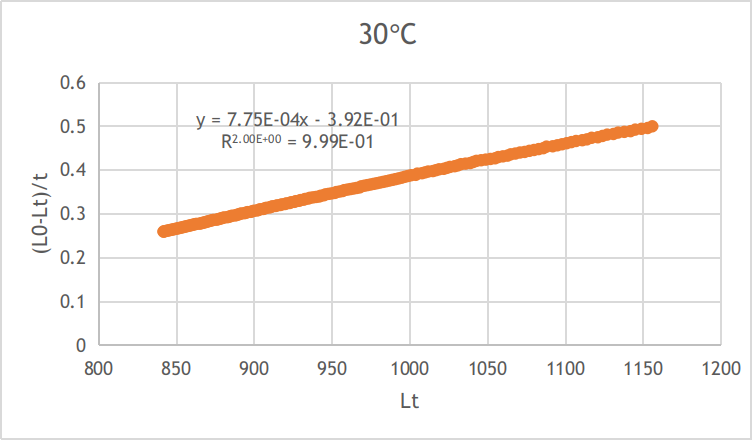
\includegraphics[width=.9\linewidth]{../img/picture-30.png}
\end{center}

得
\[
k_{1}=\frac{b}{a}=\frac{7.75\times 10^{-4}}{5.24\times 10^{-3}}=0.148mol/(dm^{3}\cdot s)
\]
\subsubsection{35摄氏度}
\label{sec:orgbcf5a1a}
T=35°C时,(L\textsubscript{0}-L\textsubscript{t})/t 对 L\textsubscript{t} 作图如下, 为了总结出线性规律, 本图舍去了前50个数据:
\begin{center}
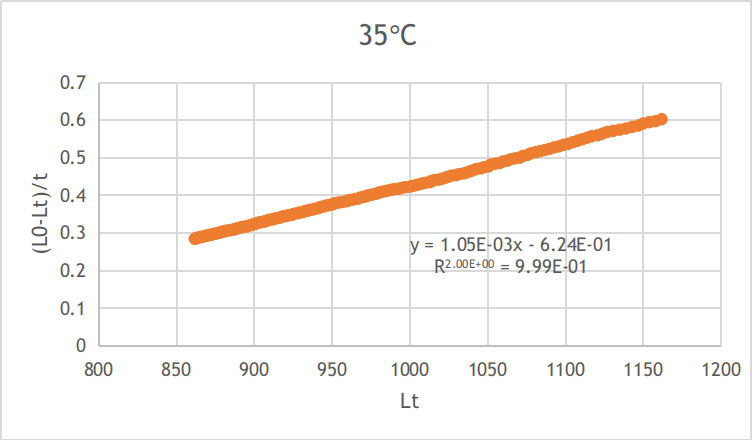
\includegraphics[width=.9\linewidth]{../img/picture-35.png}
\end{center}

得
\[
k_{2}=\frac{b}{a}=\frac{1.05\times 10^{-3}}{5.24\times 10^{-3}}=0.200mol/(dm^{3}\cdot s)
\]

\subsubsection{活化能}
\label{sec:org4c7c8e2}

由
\[
ln\frac{k_{2}}{k_{1}}=\frac{E_{a}}{R}(\frac{T_{2}-T_{1}}{T_{1}T_{2}})
\]
得
\[
E_{a}=R\cdot ln\frac{k_{2}}{k_{1}}(\frac{T_{1}\cdot T_{2}}{T_{2}-T_{1}})=68.21kJ/mol
\]

\subsection{实验讨论}
\label{sec:orgca39921}
\begin{enumerate}
\item 由(L\textsubscript{0}-L\textsubscript{t})/t 与L\textsubscript{t}关系图可知,从反应后约1-2分钟开始至反应结束,曲线图近似呈线性关系,由 \(\frac{L_{0}-L_{t}}{t}=akL_{t}-akL_{\infty}\) 可知直线斜率为ak,由此可以算出k 值。由于公式是在已假设该反应为二级反应的基础上推导得出的,而现在实验结果与理论基本一致,故该图验证了乙酸乙酯皂化反应为二级反应。
\item 由T=30°C,35°C的图比较可知,升温有利该反应的进行。事实上,对绝大多数化学反应来说,升高温度都会较大程度的提高反应速率,平均温度每升高10°C,反应速率提高2\textasciitilde{}4倍。
\item 反应开始阶段斜率为负,且不成线性,可能是由于本反应为吸热反应,开始时温度会有所降低,起始段数据作得的曲线反映的是略低温度下的 k 值;此外,可能是反应刚开始,乙酸乙酯还没有被混合均匀,局部浓度过高的缘故。故以上两种原因导致实验结果与实际 k 值有所差距,舍弃该段数据拟合。
\item 乙酸乙酯皂化反应化学方法测定的速率常数——文献值为0.1070\(mol\cdot dm^{-3}\cdot s^{-1}\),可以看出本实验结果与文献值还是有一定偏差的,现分析误差来源如下:
\begin{itemize}
\item 由于反应初期阶段t值较小,而且电导率仪还不是很稳定。故电导率测量的误差以及t值小的缘故将会给(L\textsubscript{0} – L\textsubscript{t})/t带来较大误差,从而影响到图线的拟合,进一步影响到k值的计算。
\item 由于NaOH溶液会吸收空气中的CO\textsubscript{2},而使其浓度发生变化,而在滴定NaOH溶液时,时间较长,由于吸收CO\textsubscript{2},故会影响滴定数据的准确性,进而影响加入乙酸乙酯的量。又由于皂化反应过程中NaOH溶液还在不断吸收CO\textsubscript{2},故也会影响实际参与皂化反应的NaOH溶液的量。
\item 在用移液管加入NaOH和乙酸乙酯时,操作中移液管口一不小心很容易碰触到玻璃套,这样就会造成损失,从而也会对实验结果带来误差。
\item 实验仪器的精确性也会给实验带来误差。电导率仪的反应时间是\textpm{} 0.5\%(Fs),对于乙酸乙酯皂化的缓慢反应来说可忽略不记;移液管、滴定管等仪器也有一定的误差,在操作中难免带来误差,影响初始浓度,造成k值偏差。
\item 乙酸乙酯皂化为有机反应,反应过程复杂难以预知,水溶液中电导率的情况也较复杂,相同条件下重复实验测得的电导率值会有较大差别。
\end{itemize}
\item 由本实验我们也可以知道,对于动力学的研究,物理量及实验仪器的选择应该从以下几个方面考虑:
\begin{itemize}
\item 反应前后体系的物理量变化显著;
\item 测的物质浓度成线性关系的特征物理量为最佳。
\end{itemize}
\end{enumerate}
\section{参考文献}
\label{sec:orgdaea1b7}
[1]  傅献彩,沈文霞,姚天扬.物理化学.第五版.北京:高等教育出版社,2006.1
[2]  复旦大学等编. 物理化学实验(上册)[M].北京:高等教育出版社,1979
[3] 崔献英,柯燕雄,单绍纯.物理化学实验[M].合肥:中国科学技术大学出版社,2000.4

\section{附录: 实验数据记录与处理}
\label{sec:org6a1f341}

\subsection{NaOH溶液浓度的计算}
\label{sec:orge244b9e}
\begin{center}
\begin{tabular}{lrrr}
编号 & 1 & 2 & 3\\
\hline
邻苯二甲酸氢钾(mg) & 24.3 & 28.1 & 26.4\\
NaOH用量(ml) & 22.65 & 26.24 & 24.70\\
浓度(M) & 0.00525 & 0.00524 & 0.00523\\
\end{tabular}
\end{center}

得出NaOH的浓度为0.00524M


\subsection{加入乙酸乙酯体积的计算}
\label{sec:orgfb99348}
\[
V=\frac{C_{NaOH}\times V_{NaOH}\times M}{\rho}=\frac{5.24\times 10^{-6}\times 100 \times 88.11}{0.9}=51.3\mu L
\]



\subsection{计算反应速率常数k}
\label{sec:orgebdb8d2}
\subsubsection{T=30°C=303.15K}
\label{sec:orga64e66d}
\begin{enumerate}
\item L\textsubscript{0}的测定
\label{sec:orgd13659a}

\begin{center}
\begin{tabular}{l|lp{3cm}r|l}
电脑时间 & 电导率 & 电导率单位 & 温度 & 温度单位\\
\hline
15:42:12 & 1404 & μS/cm & 27.7 & °C\\
15:43:12 & 1407 & μS/cm & 28.8 & °C\\
15:44:13 & 1407 & μS/cm & 29.2 & °C\\
15:45:13 & 1407 & μS/cm & 29.5 & °C\\
15:46:13 & 1407 & μS/cm & 29.7 & °C\\
15:47:14 & 1407 & μS/cm & 29.9 & °C\\
15:48:14 & 1407 & μS/cm & 30 & °C\\
15:49:15 & 1407 & μS/cm & 30.1 & °C\\
15:50:15 & 1407 & μS/cm & 30.1 & °C\\
15:51:15 & 1406 & μS/cm & 30.2 & °C\\
15:52:15 & 1406 & μS/cm & 30.3 & °C\\
15:53:16 & 1404 & μS/cm & 30.3 & °C\\
15:54:16 & 1404 & μS/cm & 30.3 & °C\\
15:55:16 & 1404 & μS/cm & 30.4 & °C\\
15:56:16 & 1403 & μS/cm & 30.4 & °C\\
15:57:17 & 1403 & μS/cm & 30.4 & °C\\
15:57:47 & 1403 & μS/cm & 30.5 & °C\\
\end{tabular}
\end{center}

\item L\textsubscript{t}的测定
\label{sec:orga1b6490}
\begin{center}
\begin{tabular}{l|lp{3cm}r|l}
电脑时间 & 电导率 & 电导率单位 & 温度 & 温度单位\\
\hline
16:00:58 & 1403 & μS/cm & 30.5 & °C\\
16:01:08 & 1404 & μS/cm & 30.2 & °C\\
16:01:18 & 1399 & μS/cm & 30.3 & °C\\
16:01:28 & 1393 & μS/cm & 30.3 & °C\\
16:01:38 & 1387 & μS/cm & 30.3 & °C\\
16:01:48 & 1382 & μS/cm & 30.3 & °C\\
16:01:58 & 1375 & μS/cm & 30.3 & °C\\
16:02:09 & 1369 & μS/cm & 30.3 & °C\\
16:02:18 & 1362 & μS/cm & 30.4 & °C\\
16:02:29 & 1355 & μS/cm & 30.3 & °C\\
16:02:39 & 1350 & μS/cm & 30.4 & °C\\
16:02:49 & 1343 & μS/cm & 30.4 & °C\\
16:02:59 & 1337 & μS/cm & 30.4 & °C\\
16:03:09 & 1330 & μS/cm & 30.4 & °C\\
16:03:19 & 1324 & μS/cm & 30.4 & °C\\
16:03:29 & 1318 & μS/cm & 30.4 & °C\\
16:03:39 & 1313 & μS/cm & 30.4 & °C\\
16:03:49 & 1307 & μS/cm & 30.4 & °C\\
16:04:00 & 1301 & μS/cm & 30.4 & °C\\
16:04:09 & 1295 & μS/cm & 30.4 & °C\\
16:04:20 & 1289 & μS/cm & 30.4 & °C\\
16:04:29 & 1284 & μS/cm & 30.4 & °C\\
16:04:40 & 1279 & μS/cm & 30.4 & °C\\
16:04:50 & 1273 & μS/cm & 30.4 & °C\\
16:05:00 & 1268 & μS/cm & 30.4 & °C\\
16:05:10 & 1262 & μS/cm & 30.4 & °C\\
16:05:20 & 1257 & μS/cm & 30.5 & °C\\
16:05:30 & 1253 & μS/cm & 30.5 & °C\\
16:05:40 & 1247 & μS/cm & 30.5 & °C\\
16:05:50 & 1242 & μS/cm & 30.5 & °C\\
16:06:00 & 1237 & μS/cm & 30.5 & °C\\
16:06:10 & 1232 & μS/cm & 30.5 & °C\\
16:06:20 & 1228 & μS/cm & 30.5 & °C\\
16:06:30 & 1223 & μS/cm & 30.5 & °C\\
16:06:41 & 1219 & μS/cm & 30.5 & °C\\
16:06:50 & 1214 & μS/cm & 30.5 & °C\\
\end{tabular}
\end{center}


\begin{center}
\begin{tabular}{rrlrl}
电脑时间 & 电导率 & 电导率单位 & 温度 & 温度单位\\
\hline
16:07:01 & 1210 & μS/cm & 30.5 & °C\\
16:07:11 & 1206 & μS/cm & 30.5 & °C\\
16:07:21 & 1201 & μS/cm & 30.5 & °C\\
16:07:31 & 1197 & μS/cm & 30.5 & °C\\
16:07:41 & 1192 & μS/cm & 30.5 & °C\\
16:07:51 & 1188 & μS/cm & 30.5 & °C\\
16:08:01 & 1184 & μS/cm & 30.5 & °C\\
16:08:11 & 1180 & μS/cm & 30.5 & °C\\
16:08:21 & 1176 & μS/cm & 30.5 & °C\\
16:08:31 & 1172 & μS/cm & 30.5 & °C\\
16:08:41 & 1168 & μS/cm & 30.5 & °C\\
16:08:52 & 1164 & μS/cm & 30.5 & °C\\
16:09:01 & 1160 & μS/cm & 30.5 & °C\\
16:09:12 & 1156 & μS/cm & 30.5 & °C\\
16:09:22 & 1153 & μS/cm & 30.5 & °C\\
16:09:32 & 1149 & μS/cm & 30.5 & °C\\
16:09:42 & 1145 & μS/cm & 30.5 & °C\\
16:09:52 & 1142 & μS/cm & 30.5 & °C\\
16:10:02 & 1138 & μS/cm & 30.5 & °C\\
16:10:12 & 1134 & μS/cm & 30.5 & °C\\
16:10:22 & 1131 & μS/cm & 30.6 & °C\\
16:10:32 & 1127 & μS/cm & 30.5 & °C\\
16:10:42 & 1124 & μS/cm & 30.6 & °C\\
16:10:52 & 1121 & μS/cm & 30.6 & °C\\
16:11:02 & 1117 & μS/cm & 30.6 & °C\\
16:11:13 & 1114 & μS/cm & 30.5 & °C\\
16:11:22 & 1111 & μS/cm & 30.6 & °C\\
16:11:33 & 1107 & μS/cm & 30.6 & °C\\
16:11:43 & 1104 & μS/cm & 30.6 & °C\\
16:11:53 & 1101 & μS/cm & 30.6 & °C\\
16:12:03 & 1098 & μS/cm & 30.6 & °C\\
16:12:13 & 1095 & μS/cm & 30.6 & °C\\
16:12:23 & 1092 & μS/cm & 30.6 & °C\\
16:12:33 & 1088 & μS/cm & 30.6 & °C\\
16:12:43 & 1086 & μS/cm & 30.6 & °C\\
16:12:53 & 1083 & μS/cm & 30.6 & °C\\
16:13:03 & 1080 & μS/cm & 30.6 & °C\\
16:13:13 & 1077 & μS/cm & 30.6 & °C\\
16:13:24 & 1074 & μS/cm & 30.6 & °C\\
16:13:33 & 1071 & μS/cm & 30.6 & °C\\
16:13:44 & 1068 & μS/cm & 30.6 & °C\\
16:13:54 & 1065 & μS/cm & 30.6 & °C\\
16:14:04 & 1063 & μS/cm & 30.6 & °C\\
16:14:14 & 1060 & μS/cm & 30.6 & °C\\
16:14:24 & 1057 & μS/cm & 30.6 & °C\\
16:14:34 & 1055 & μS/cm & 30.6 & °C\\
16:14:44 & 1052 & μS/cm & 30.6 & °C\\
16:14:54 & 1049 & μS/cm & 30.6 & °C\\
\end{tabular}
\end{center}

\begin{center}
\begin{tabular}{rrlrl}
电脑时间 & 电导率 & 电导率单位 & 温度 & 温度单位\\
\hline
16:15:04 & 1046 & μS/cm & 30.6 & °C\\
16:15:14 & 1043 & μS/cm & 30.6 & °C\\
16:15:24 & 1041 & μS/cm & 30.6 & °C\\
16:15:34 & 1039 & μS/cm & 30.6 & °C\\
16:15:44 & 1036 & μS/cm & 30.6 & °C\\
16:15:54 & 1033 & μS/cm & 30.6 & °C\\
16:16:05 & 1031 & μS/cm & 30.6 & °C\\
16:16:14 & 1029 & μS/cm & 30.6 & °C\\
16:16:25 & 1026 & μS/cm & 30.6 & °C\\
16:16:35 & 1024 & μS/cm & 30.6 & °C\\
16:16:45 & 1022 & μS/cm & 30.6 & °C\\
16:16:55 & 1019 & μS/cm & 30.6 & °C\\
16:17:05 & 1017 & μS/cm & 30.6 & °C\\
16:17:15 & 1015 & μS/cm & 30.6 & °C\\
16:17:25 & 1012 & μS/cm & 30.6 & °C\\
16:17:35 & 1010 & μS/cm & 30.7 & °C\\
16:17:45 & 1008 & μS/cm & 30.7 & °C\\
16:17:55 & 1005 & μS/cm & 30.7 & °C\\
16:18:05 & 1004 & μS/cm & 30.7 & °C\\
16:18:15 & 1001 & μS/cm & 30.7 & °C\\
16:18:25 & 999 & μS/cm & 30.6 & °C\\
16:18:35 & 997 & μS/cm & 30.7 & °C\\
16:18:46 & 995 & μS/cm & 30.7 & °C\\
16:18:56 & 993 & μS/cm & 30.7 & °C\\
16:19:06 & 991 & μS/cm & 30.7 & °C\\
16:19:16 & 989 & μS/cm & 30.7 & °C\\
16:19:26 & 987 & μS/cm & 30.7 & °C\\
16:19:36 & 985 & μS/cm & 30.7 & °C\\
16:19:46 & 983 & μS/cm & 30.7 & °C\\
16:19:56 & 981 & μS/cm & 30.7 & °C\\
16:20:06 & 979 & μS/cm & 30.7 & °C\\
16:20:16 & 977 & μS/cm & 30.7 & °C\\
16:20:26 & 975 & μS/cm & 30.7 & °C\\
16:20:36 & 973 & μS/cm & 30.7 & °C\\
16:20:46 & 971 & μS/cm & 30.7 & °C\\
16:20:56 & 969 & μS/cm & 30.7 & °C\\
16:21:07 & 968 & μS/cm & 30.7 & °C\\
16:21:17 & 966 & μS/cm & 30.7 & °C\\
16:21:27 & 964 & μS/cm & 30.7 & °C\\
16:21:37 & 962 & μS/cm & 30.7 & °C\\
16:21:47 & 960 & μS/cm & 30.7 & °C\\
16:21:57 & 958 & μS/cm & 30.7 & °C\\
\end{tabular}
\end{center}

\begin{center}
\begin{tabular}{rrlrl}
电脑时间 & 电导率 & 电导率单位 & 温度 & 温度单位\\
\hline
16:22:07 & 957 & μS/cm & 30.7 & °C\\
16:22:17 & 955 & μS/cm & 30.7 & °C\\
16:22:27 & 953 & μS/cm & 30.7 & °C\\
16:22:37 & 952 & μS/cm & 30.7 & °C\\
16:22:47 & 950 & μS/cm & 30.7 & °C\\
16:22:57 & 948 & μS/cm & 30.7 & °C\\
16:23:07 & 946 & μS/cm & 30.7 & °C\\
16:23:18 & 945 & μS/cm & 30.7 & °C\\
16:23:28 & 943 & μS/cm & 30.7 & °C\\
16:23:38 & 942 & μS/cm & 30.7 & °C\\
16:23:48 & 940 & μS/cm & 30.7 & °C\\
16:23:58 & 938 & μS/cm & 30.7 & °C\\
16:24:08 & 936 & μS/cm & 30.7 & °C\\
16:24:18 & 935 & μS/cm & 30.7 & °C\\
16:24:28 & 933 & μS/cm & 30.7 & °C\\
16:24:38 & 932 & μS/cm & 30.7 & °C\\
16:24:48 & 930 & μS/cm & 30.7 & °C\\
16:24:58 & 929 & μS/cm & 30.7 & °C\\
16:25:08 & 927 & μS/cm & 30.8 & °C\\
16:25:18 & 926 & μS/cm & 30.8 & °C\\
16:25:28 & 924 & μS/cm & 30.8 & °C\\
16:25:39 & 923 & μS/cm & 30.8 & °C\\
16:25:49 & 921 & μS/cm & 30.8 & °C\\
16:25:59 & 920 & μS/cm & 30.8 & °C\\
16:26:09 & 918 & μS/cm & 30.8 & °C\\
16:26:19 & 917 & μS/cm & 30.8 & °C\\
16:26:29 & 915 & μS/cm & 30.8 & °C\\
16:26:39 & 914 & μS/cm & 30.8 & °C\\
16:26:49 & 912 & μS/cm & 30.8 & °C\\
16:26:59 & 911 & μS/cm & 30.8 & °C\\
16:27:09 & 910 & μS/cm & 30.8 & °C\\
16:27:19 & 908 & μS/cm & 30.8 & °C\\
16:27:29 & 907 & μS/cm & 30.8 & °C\\
16:27:39 & 906 & μS/cm & 30.8 & °C\\
16:27:49 & 904 & μS/cm & 30.8 & °C\\
16:28:00 & 903 & μS/cm & 30.8 & °C\\
16:28:10 & 902 & μS/cm & 30.8 & °C\\
16:28:20 & 900 & μS/cm & 30.8 & °C\\
16:28:30 & 899 & μS/cm & 30.8 & °C\\
16:28:40 & 898 & μS/cm & 30.8 & °C\\
16:28:50 & 896 & μS/cm & 30.8 & °C\\
\end{tabular}
\end{center}

\begin{center}
\begin{tabular}{rrlrl}
电脑时间 & 电导率 & 电导率单位 & 温度 & 温度单位\\
\hline
16:29:00 & 895 & μS/cm & 30.8 & °C\\
16:29:10 & 894 & μS/cm & 30.8 & °C\\
16:29:20 & 892 & μS/cm & 30.8 & °C\\
16:29:30 & 891 & μS/cm & 30.8 & °C\\
16:29:40 & 890 & μS/cm & 30.8 & °C\\
16:29:50 & 889 & μS/cm & 30.8 & °C\\
16:30:00 & 888 & μS/cm & 30.8 & °C\\
16:30:10 & 886 & μS/cm & 30.8 & °C\\
16:30:21 & 885 & μS/cm & 30.8 & °C\\
16:30:31 & 884 & μS/cm & 30.8 & °C\\
16:30:41 & 883 & μS/cm & 30.8 & °C\\
16:30:51 & 881 & μS/cm & 30.8 & °C\\
16:31:01 & 880 & μS/cm & 30.8 & °C\\
16:31:11 & 879 & μS/cm & 30.8 & °C\\
16:31:21 & 878 & μS/cm & 30.9 & °C\\
16:31:31 & 877 & μS/cm & 30.8 & °C\\
16:31:41 & 876 & μS/cm & 30.8 & °C\\
16:31:51 & 874 & μS/cm & 30.9 & °C\\
16:32:01 & 873 & μS/cm & 30.8 & °C\\
16:32:11 & 872 & μS/cm & 30.8 & °C\\
16:32:21 & 871 & μS/cm & 30.9 & °C\\
16:32:31 & 870 & μS/cm & 30.9 & °C\\
16:32:42 & 869 & μS/cm & 30.9 & °C\\
16:32:52 & 868 & μS/cm & 30.9 & °C\\
16:33:02 & 867 & μS/cm & 30.8 & °C\\
16:33:12 & 866 & μS/cm & 30.9 & °C\\
16:33:22 & 865 & μS/cm & 30.9 & °C\\
16:33:32 & 863 & μS/cm & 30.9 & °C\\
16:33:42 & 862 & μS/cm & 30.9 & °C\\
16:33:52 & 861 & μS/cm & 30.9 & °C\\
16:34:02 & 860 & μS/cm & 30.9 & °C\\
16:34:12 & 859 & μS/cm & 30.9 & °C\\
16:34:22 & 858 & μS/cm & 30.9 & °C\\
16:34:32 & 857 & μS/cm & 30.9 & °C\\
16:34:42 & 856 & μS/cm & 30.9 & °C\\
16:34:52 & 855 & μS/cm & 30.9 & °C\\
16:35:03 & 854 & μS/cm & 30.9 & °C\\
16:35:13 & 853 & μS/cm & 30.9 & °C\\
16:35:23 & 852 & μS/cm & 30.9 & °C\\
16:35:33 & 851 & μS/cm & 30.9 & °C\\
16:35:43 & 850 & μS/cm & 30.9 & °C\\
16:35:53 & 849 & μS/cm & 30.9 & °C\\
\end{tabular}
\end{center}

\begin{center}
\begin{tabular}{rrlrl}
电脑时间 & 电导率 & 电导率单位 & 温度 & 温度单位\\
\hline
16:36:03 & 848 & μS/cm & 30.9 & °C\\
16:36:13 & 847 & μS/cm & 30.9 & °C\\
16:36:23 & 846 & μS/cm & 30.9 & °C\\
16:36:33 & 845 & μS/cm & 30.9 & °C\\
16:36:43 & 844 & μS/cm & 30.9 & °C\\
16:36:54 & 843 & μS/cm & 30.9 & °C\\
16:37:03 & 842 & μS/cm & 30.9 & °C\\
16:37:08 & 842 & μS/cm & 30.9 & °C\\
\end{tabular}
\end{center}

(L\textsubscript{0}‐L\textsubscript{t})/t 对 L\textsubscript{t} 作图如下:
\begin{center}
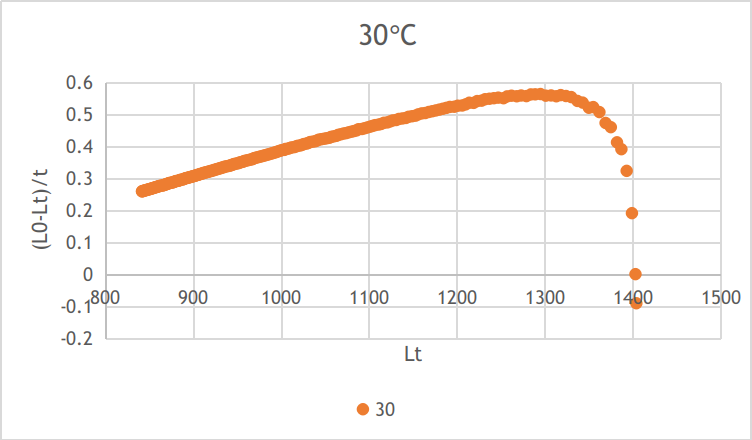
\includegraphics[width=.9\linewidth]{../img/picture-30-1.png}
\end{center}
\end{enumerate}

\subsubsection{T=35°C=308.15K}
\label{sec:orge89a038}
\begin{enumerate}
\item L\textsubscript{0}的测定
\label{sec:org101eb75}
\begin{center}
\begin{tabular}{l|lp{3cm}r|l}
电脑时间 & 电导率 & 电导率单位 & 温度 & 温度单位\\
\hline
16:50:40 & 1375 & μS/cm & 25.9 & °C\\
16:51:41 & 1416 & μS/cm & 28.7 & °C\\
16:52:41 & 1430 & μS/cm & 29.8 & °C\\
16:53:41 & 1439 & μS/cm & 30.6 & °C\\
16:54:42 & 1446 & μS/cm & 31.2 & °C\\
16:55:42 & 1450 & μS/cm & 31.7 & °C\\
16:56:42 & 1453 & μS/cm & 32.1 & °C\\
16:57:43 & 1455 & μS/cm & 32.3 & °C\\
16:58:43 & 1457 & μS/cm & 32.6 & °C\\
16:59:43 & 1458 & μS/cm & 32.8 & °C\\
17:00:44 & 1460 & μS/cm & 32.9 & °C\\
17:01:44 & 1462 & μS/cm & 33.1 & °C\\
17:02:44 & 1465 & μS/cm & 33.2 & °C\\
17:03:45 & 1463 & μS/cm & 33.3 & °C\\
17:04:45 & 1459 & μS/cm & 33.4 & °C\\
17:05:45 & 1463 & μS/cm & 33.5 & °C\\
17:06:45 & 1464 & μS/cm & 33.6 & °C\\
17:07:46 & 1463 & μS/cm & 33.6 & °C\\
17:08:46 & 1458 & μS/cm & 33.7 & °C\\
17:09:46 & 1461 & μS/cm & 33.7 & °C\\
17:10:47 & 1462 & μS/cm & 33.8 & °C\\
17:11:47 & 1451 & μS/cm & 33.8 & °C\\
17:12:47 & 1451 & μS/cm & 33.8 & °C\\
17:13:48 & 1458 & μS/cm & 33.9 & °C\\
17:13:56 & 1459 & μS/cm & 33.9 & °C\\
\end{tabular}
\end{center}
\item L\textsubscript{t}的测定
\label{sec:orgced6ae1}
\begin{center}
\begin{tabular}{l|lp{3cm}r|l}
电脑时间 & 电导率 & 电导率单位 & 温度 & 温度单位\\
\hline
17:16:43 & 1459 & μS/cm & 33.9 & °C\\
17:16:53 & 1457 & μS/cm & 34 & °C\\
17:17:03 & 1444 & μS/cm & 34 & °C\\
17:17:13 & 1437 & μS/cm & 34 & °C\\
17:17:23 & 1431 & μS/cm & 34 & °C\\
17:17:33 & 1425 & μS/cm & 34 & °C\\
17:17:43 & 1421 & μS/cm & 34 & °C\\
17:17:53 & 1415 & μS/cm & 34 & °C\\
17:18:03 & 1399 & μS/cm & 34 & °C\\
17:18:13 & 1390 & μS/cm & 34 & °C\\
17:18:23 & 1385 & μS/cm & 34 & °C\\
17:18:33 & 1380 & μS/cm & 34 & °C\\
17:18:44 & 1373 & μS/cm & 34 & °C\\
17:18:53 & 1368 & μS/cm & 34 & °C\\
17:19:04 & 1356 & μS/cm & 34 & °C\\
17:19:14 & 1346 & μS/cm & 34 & °C\\
17:19:24 & 1339 & μS/cm & 34 & °C\\
17:19:34 & 1332 & μS/cm & 34 & °C\\
17:19:44 & 1320 & μS/cm & 34 & °C\\
17:19:54 & 1313 & μS/cm & 34 & °C\\
17:20:04 & 1307 & μS/cm & 34 & °C\\
17:20:14 & 1300 & μS/cm & 34 & °C\\
17:20:24 & 1292 & μS/cm & 34 & °C\\
17:20:35 & 1286 & μS/cm & 34 & °C\\
17:20:44 & 1281 & μS/cm & 34 & °C\\
17:20:54 & 1276 & μS/cm & 34 & °C\\
17:21:04 & 1268 & μS/cm & 34 & °C\\
17:21:14 & 1261 & μS/cm & 34 & °C\\
17:21:25 & 1256 & μS/cm & 34 & °C\\
17:21:35 & 1250 & μS/cm & 34 & °C\\
17:21:45 & 1245 & μS/cm & 34 & °C\\
17:21:55 & 1240 & μS/cm & 34 & °C\\
17:22:05 & 1235 & μS/cm & 34 & °C\\
17:22:15 & 1230 & μS/cm & 34 & °C\\
17:22:25 & 1225 & μS/cm & 34 & °C\\
17:22:35 & 1220 & μS/cm & 34 & °C\\
17:22:45 & 1216 & μS/cm & 34.1 & °C\\
17:22:55 & 1212 & μS/cm & 34.1 & °C\\
17:23:05 & 1207 & μS/cm & 34.1 & °C\\
17:23:16 & 1202 & μS/cm & 34.1 & °C\\
17:23:25 & 1199 & μS/cm & 34.1 & °C\\
17:23:36 & 1194 & μS/cm & 34.1 & °C\\
17:23:46 & 1190 & μS/cm & 34.1 & °C\\
17:23:56 & 1186 & μS/cm & 34.1 & °C\\
\end{tabular}
\end{center}

\begin{center}
\begin{tabular}{rrlrl}
电脑时间 & 电导率 & 电导率单位 & 温度 & 温度单位\\
\hline
17:24:06 & 1182 & μS/cm & 34.1 & °C\\
17:24:16 & 1177 & μS/cm & 34.1 & °C\\
17:24:26 & 1173 & μS/cm & 34.1 & °C\\
17:24:36 & 1169 & μS/cm & 34.1 & °C\\
17:24:46 & 1166 & μS/cm & 34.1 & °C\\
17:24:56 & 1162 & μS/cm & 34.1 & °C\\
17:25:07 & 1158 & μS/cm & 34.1 & °C\\
17:25:16 & 1154 & μS/cm & 34.1 & °C\\
17:25:26 & 1150 & μS/cm & 34.1 & °C\\
17:25:36 & 1147 & μS/cm & 34.1 & °C\\
17:25:46 & 1143 & μS/cm & 34.1 & °C\\
17:25:57 & 1139 & μS/cm & 34.1 & °C\\
17:26:07 & 1135 & μS/cm & 34.1 & °C\\
17:26:17 & 1131 & μS/cm & 34.1 & °C\\
17:26:27 & 1127 & μS/cm & 34.1 & °C\\
17:26:37 & 1124 & μS/cm & 34.1 & °C\\
17:26:47 & 1121 & μS/cm & 34.1 & °C\\
17:26:57 & 1117 & μS/cm & 34.1 & °C\\
17:27:07 & 1114 & μS/cm & 34.1 & °C\\
17:27:17 & 1111 & μS/cm & 34.1 & °C\\
17:27:27 & 1108 & μS/cm & 34.1 & °C\\
17:27:37 & 1105 & μS/cm & 34.1 & °C\\
17:27:48 & 1102 & μS/cm & 34.1 & °C\\
17:27:57 & 1099 & μS/cm & 34.1 & °C\\
17:28:08 & 1096 & μS/cm & 34.1 & °C\\
17:28:17 & 1093 & μS/cm & 34.1 & °C\\
17:28:28 & 1090 & μS/cm & 34.1 & °C\\
17:28:38 & 1087 & μS/cm & 34.1 & °C\\
17:28:48 & 1084 & μS/cm & 34.1 & °C\\
17:28:58 & 1081 & μS/cm & 34.1 & °C\\
17:29:08 & 1078 & μS/cm & 34.1 & °C\\
17:29:18 & 1076 & μS/cm & 34.1 & °C\\
17:29:28 & 1073 & μS/cm & 34.1 & °C\\
17:29:39 & 1071 & μS/cm & 34.1 & °C\\
17:29:48 & 1068 & μS/cm & 34.1 & °C\\
17:29:58 & 1065 & μS/cm & 34.1 & °C\\
17:30:08 & 1063 & μS/cm & 34.1 & °C\\
17:30:18 & 1060 & μS/cm & 34.1 & °C\\
17:30:29 & 1058 & μS/cm & 34.1 & °C\\
17:30:38 & 1055 & μS/cm & 34.1 & °C\\
17:30:49 & 1052 & μS/cm & 34.1 & °C\\
17:30:59 & 1051 & μS/cm & 34.1 & °C\\
\end{tabular}
\end{center}

\begin{center}
\begin{tabular}{rrlrl}
电脑时间 & 电导率 & 电导率单位 & 温度 & 温度单位\\
\hline
17:31:09 & 1048 & μS/cm & 34.1 & °C\\
17:31:19 & 1046 & μS/cm & 34.2 & °C\\
17:31:29 & 1043 & μS/cm & 34.1 & °C\\
17:31:39 & 1041 & μS/cm & 34.1 & °C\\
17:31:49 & 1039 & μS/cm & 34.1 & °C\\
17:31:59 & 1037 & μS/cm & 34.1 & °C\\
17:32:09 & 1035 & μS/cm & 34.1 & °C\\
17:32:19 & 1032 & μS/cm & 34.2 & °C\\
17:32:29 & 1030 & μS/cm & 34.1 & °C\\
17:32:39 & 1027 & μS/cm & 34.1 & °C\\
17:32:49 & 1025 & μS/cm & 34.1 & °C\\
17:33:00 & 1023 & μS/cm & 34.2 & °C\\
17:33:10 & 1021 & μS/cm & 34.2 & °C\\
17:33:20 & 1019 & μS/cm & 34.2 & °C\\
17:33:30 & 1016 & μS/cm & 34.2 & °C\\
17:33:40 & 1014 & μS/cm & 34.2 & °C\\
17:33:50 & 1013 & μS/cm & 34.2 & °C\\
17:34:00 & 1010 & μS/cm & 34.2 & °C\\
17:34:10 & 1008 & μS/cm & 34.2 & °C\\
17:34:20 & 1006 & μS/cm & 34.2 & °C\\
17:34:30 & 1004 & μS/cm & 34.2 & °C\\
17:34:40 & 1002 & μS/cm & 34.2 & °C\\
17:34:50 & 1000 & μS/cm & 34.2 & °C\\
17:35:00 & 997 & μS/cm & 34.2 & °C\\
17:35:10 & 995 & μS/cm & 34.2 & °C\\
17:35:21 & 993 & μS/cm & 34.2 & °C\\
17:35:31 & 990 & μS/cm & 34.2 & °C\\
17:35:41 & 988 & μS/cm & 34.2 & °C\\
17:35:51 & 986 & μS/cm & 34.2 & °C\\
17:36:01 & 984 & μS/cm & 34.2 & °C\\
17:36:11 & 982 & μS/cm & 34.2 & °C\\
17:36:21 & 980 & μS/cm & 34.2 & °C\\
17:36:31 & 979 & μS/cm & 34.2 & °C\\
17:36:41 & 977 & μS/cm & 34.2 & °C\\
17:36:51 & 975 & μS/cm & 34.2 & °C\\
17:37:01 & 973 & μS/cm & 34.2 & °C\\
17:37:11 & 972 & μS/cm & 34.2 & °C\\
17:37:21 & 970 & μS/cm & 34.2 & °C\\
17:37:32 & 968 & μS/cm & 34.2 & °C\\
17:37:42 & 967 & μS/cm & 34.2 & °C\\
17:37:52 & 965 & μS/cm & 34.2 & °C\\
\end{tabular}
\end{center}

\begin{center}
\begin{tabular}{rrlrl}
电脑时间 & 电导率 & 电导率单位 & 温度 & 温度单位\\
\hline
17:38:02 & 963 & μS/cm & 34.2 & °C\\
17:38:12 & 961 & μS/cm & 34.2 & °C\\
17:38:22 & 960 & μS/cm & 34.2 & °C\\
17:38:32 & 958 & μS/cm & 34.2 & °C\\
17:38:42 & 956 & μS/cm & 34.2 & °C\\
17:38:52 & 954 & μS/cm & 34.2 & °C\\
17:39:02 & 952 & μS/cm & 34.2 & °C\\
17:39:12 & 951 & μS/cm & 34.2 & °C\\
17:39:22 & 950 & μS/cm & 34.2 & °C\\
17:39:32 & 948 & μS/cm & 34.2 & °C\\
17:39:42 & 946 & μS/cm & 34.2 & °C\\
17:39:53 & 945 & μS/cm & 34.2 & °C\\
17:40:03 & 943 & μS/cm & 34.2 & °C\\
17:40:13 & 942 & μS/cm & 34.2 & °C\\
17:40:23 & 941 & μS/cm & 34.2 & °C\\
17:40:33 & 939 & μS/cm & 34.2 & °C\\
17:40:43 & 938 & μS/cm & 34.2 & °C\\
17:40:53 & 936 & μS/cm & 34.2 & °C\\
17:41:03 & 935 & μS/cm & 34.2 & °C\\
17:41:13 & 933 & μS/cm & 34.2 & °C\\
17:41:23 & 932 & μS/cm & 34.2 & °C\\
17:41:33 & 931 & μS/cm & 34.2 & °C\\
17:41:43 & 929 & μS/cm & 34.2 & °C\\
17:41:53 & 928 & μS/cm & 34.2 & °C\\
17:42:04 & 926 & μS/cm & 34.2 & °C\\
17:42:14 & 925 & μS/cm & 34.2 & °C\\
17:42:24 & 924 & μS/cm & 34.2 & °C\\
17:42:34 & 922 & μS/cm & 34.2 & °C\\
17:42:44 & 921 & μS/cm & 34.2 & °C\\
17:42:54 & 919 & μS/cm & 34.2 & °C\\
17:43:04 & 918 & μS/cm & 34.2 & °C\\
17:43:14 & 917 & μS/cm & 34.2 & °C\\
17:43:24 & 916 & μS/cm & 34.2 & °C\\
17:43:34 & 914 & μS/cm & 34.2 & °C\\
17:43:44 & 913 & μS/cm & 34.2 & °C\\
17:43:54 & 912 & μS/cm & 34.2 & °C\\
17:44:04 & 910 & μS/cm & 34.2 & °C\\
17:44:15 & 909 & μS/cm & 34.2 & °C\\
17:44:25 & 908 & μS/cm & 34.2 & °C\\
17:44:35 & 907 & μS/cm & 34.2 & °C\\
17:44:45 & 906 & μS/cm & 34.2 & °C\\
17:44:55 & 904 & μS/cm & 34.2 & °C\\
\end{tabular}
\end{center}

\begin{center}
\begin{tabular}{rrlrl}
电脑时间 & 电导率 & 电导率单位 & 温度 & 温度单位\\
\hline
17:45:05 & 903 & μS/cm & 34.2 & °C\\
17:45:15 & 902 & μS/cm & 34.2 & °C\\
17:45:25 & 901 & μS/cm & 34.2 & °C\\
17:45:35 & 900 & μS/cm & 34.2 & °C\\
17:45:45 & 899 & μS/cm & 34.2 & °C\\
17:45:55 & 898 & μS/cm & 34.2 & °C\\
17:46:05 & 897 & μS/cm & 34.2 & °C\\
17:46:15 & 896 & μS/cm & 34.2 & °C\\
17:46:25 & 895 & μS/cm & 34.2 & °C\\
17:46:36 & 893 & μS/cm & 34.2 & °C\\
17:46:46 & 892 & μS/cm & 34.2 & °C\\
17:46:56 & 891 & μS/cm & 34.2 & °C\\
17:47:06 & 890 & μS/cm & 34.2 & °C\\
17:47:16 & 889 & μS/cm & 34.2 & °C\\
17:47:26 & 888 & μS/cm & 34.2 & °C\\
17:47:36 & 887 & μS/cm & 34.2 & °C\\
17:47:46 & 886 & μS/cm & 34.2 & °C\\
17:47:56 & 885 & μS/cm & 34.2 & °C\\
17:48:06 & 883 & μS/cm & 34.2 & °C\\
17:48:16 & 882 & μS/cm & 34.2 & °C\\
17:48:26 & 881 & μS/cm & 34.2 & °C\\
17:48:36 & 880 & μS/cm & 34.2 & °C\\
17:48:47 & 879 & μS/cm & 34.2 & °C\\
17:48:57 & 878 & μS/cm & 34.2 & °C\\
17:49:07 & 877 & μS/cm & 34.2 & °C\\
17:49:17 & 876 & μS/cm & 34.2 & °C\\
17:49:27 & 875 & μS/cm & 34.2 & °C\\
17:49:37 & 874 & μS/cm & 34.2 & °C\\
17:49:47 & 873 & μS/cm & 34.2 & °C\\
17:49:57 & 872 & μS/cm & 34.2 & °C\\
17:50:07 & 871 & μS/cm & 34.2 & °C\\
17:50:17 & 870 & μS/cm & 34.2 & °C\\
17:50:27 & 869 & μS/cm & 34.2 & °C\\
17:50:37 & 868 & μS/cm & 34.2 & °C\\
17:50:47 & 867 & μS/cm & 34.2 & °C\\
17:50:58 & 866 & μS/cm & 34.2 & °C\\
17:51:08 & 865 & μS/cm & 34.2 & °C\\
17:51:18 & 864 & μS/cm & 34.2 & °C\\
17:51:28 & 863 & μS/cm & 34.2 & °C\\
17:51:38 & 863 & μS/cm & 34.2 & °C\\
17:51:46 & 862 & μS/cm & 34.2 & °C\\
\end{tabular}
\end{center}

(L\textsubscript{0}‐L\textsubscript{t})/t 对 L\textsubscript{t} 作图如下:
\begin{center}
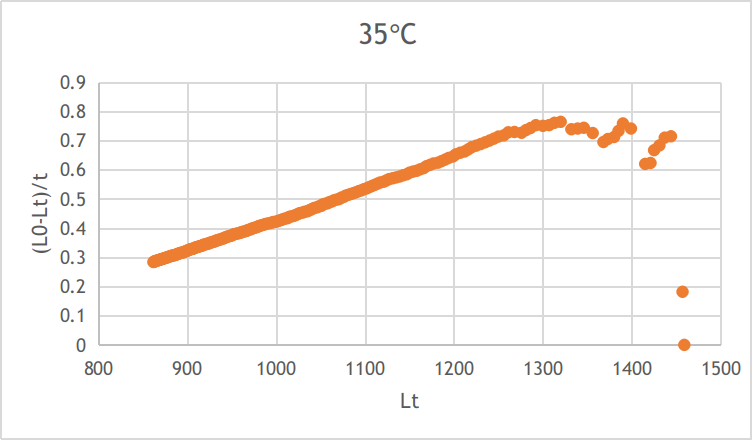
\includegraphics[width=.9\linewidth]{../img/picture-35-1.png}
\end{center}
\end{enumerate}
\end{document}
